\chapter{Literature Review}
	
\par
\hspace{0.6cm} Most of the reported level crossing ADC's suffer from the large loop delay which results in slope overloading error. Some of the authors tried to eliminate the slope overload problem in level crossing ADC's, but they end up in increasing complexity or with some other problem. Following section breifly describes the attempts made to eliminate the slope overload problem in level crossing ADC's.


\section{ Level crossing ADC}

\par
\hspace{0.6cm} Level cross sampling is best suited for asynchronous ADC's. Fig.~\ref{fig:REFA} shows a block diagram of level crossing ADC architecture~\cite{4672051}. The architecture of the level crossing ADC is a tracking loop controlled by the analog input signal $V_{in}$. It is composed of a difference quantificator, an up/down counter, a digital-to-analog converter (DAC), and a timer. Difference quantificator behaves like a window detector, when the analog input $V_{in}$ is with in the specified range both outputs $INC$ and $DCR$ from difference quantificator are zero. 

\begin{figure}[h]
	\begin{center}
		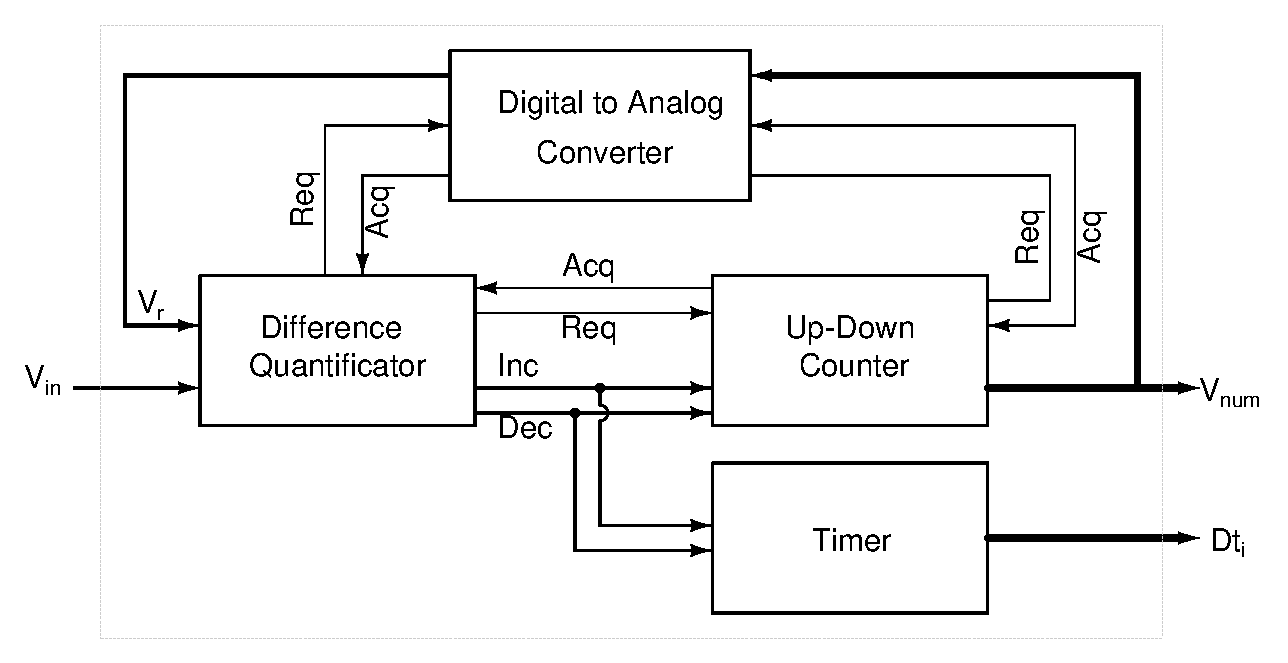
\includegraphics[scale=0.45]{./Figures/REFA.ps}
		\caption{Block Diagram of level crossing ADC.}
		\label{fig:REFA}
	\end{center}
\end{figure}

\par
\hspace{0.6cm}If the analog input $V_{in}$ crosses the specified range it generates either $INC$ or $DCR$ depending on the direction of analog input $V_{in}$. Generally the range of the difference quantificator will be +LSB to -LSB of the reference signal generated by the DAC. Up/down counter counts the number of transitions the analog input $V_{in}$ have. If the $INC$ signal from difference quantificator becomes '1' the counter contents will be incremented by one, if the $DCR$ signal generated from difference quantificator becomes '1' the contents of the counter are decremented by one, in a simplified sense the contents of the up/down counter refers to the digital value corresponding to then analog input value of the level crossing ADC. 

\par
\hspace{0.6cm} The DAC which converts the digital input form  up/down counter in to the corresponding analog value, which is used to generate the reference value for the difference quantificator. Timer is driven by high speed clock which counts the time difference between the present sample and the previous sample. All the hand shaking signals are asynchronous between the block. Once the whole operation is completed it waits till another transition occurred in the difference quantificator. 

\par
\hspace{0.6cm} 	Generally the up-down counter in level crossing ADC is implemented using an adder-subtractor circuit. As the number of bits in up-down counter increases the delay in calculating the up-down counter value increases when a trigger generated by the difference quantificator. This increase in delay results in increased loop delay of the level crossing ADC. If the loop delay of the  level crossing ADC increases, it effectively reduces the maximum frequencies in the input signal which it can track without slope overload error. 




\section{ Signal-dependent variable-resolution ADC}


\par
\hspace{0.6cm} The authors kurchuk et al have suggested signal dependent variable resolution quantization technique to reduce slope overload error. Fig.~\ref{fig:REFB} shows a block diagram of slope dependent variable resolution quantization level crossing ADC architecture~\cite{kurchuk2009signal}. In this technique a slope detector at the input of ADC is used to measure the slope of the input analog signal. Depending on the slope of the input analog signal, the controller circuit in level crossing ADC changes the resolution of the level crossing ADC. 

\begin{figure}[h]
	\begin{center}
		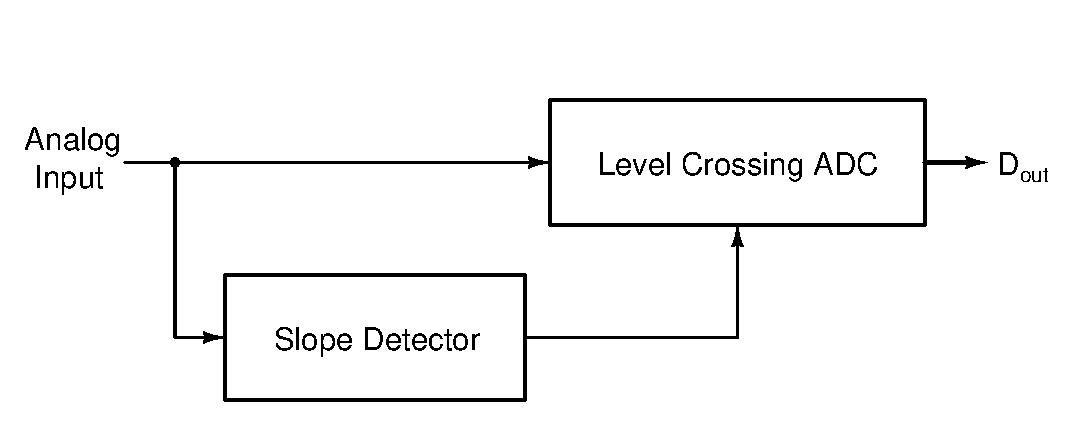
\includegraphics[scale=0.6]{./Figures/REFB.ps}
		\caption{Block Diagram of level crossing ADC.}
		\label{fig:REFB}
	\end{center}
\end{figure}

\par
\hspace{0.6cm} The effectiveness of this technique depends on how accurately the slope is measured by the input slope detector. In this technique the complexity of the level crossing ADC increases with the number of bits to represent the slope. There is some delay in the output because first the slope detector should detect the the slope then the conversion process is started.






\section{ Adaptive asynchronous ADC}

\par
\hspace{0.6cm} The authors Agarwal et al have suggested Adaptive asynchronous technique to reduce slope overload error. As the up-down counter linear fasion the autors replaced the up-down counter with the logic shown in Fig.~\ref{fig:REFC} in variable input slope dependent level crossing ADC architecture~\cite{agarwal2009adaptive}. The PSL block in block diagram is a pulse stretching logic, which is implemented with the low pass R-C filter. When any of the outputs of difference quantificator are high these PSL blocks extenend the pulse duration of the outputs of difference quantificator and the delay elements store it's value. Depending on the outputs of delay elements and outputs of the difference quantificator the increment/decrement step size is changed in controller logic. In this technique previous bits are stored, based on which the slope is estimated and the resolution of level crossing ADC is adjusted. 

\begin{figure}[h]
	\begin{center}
		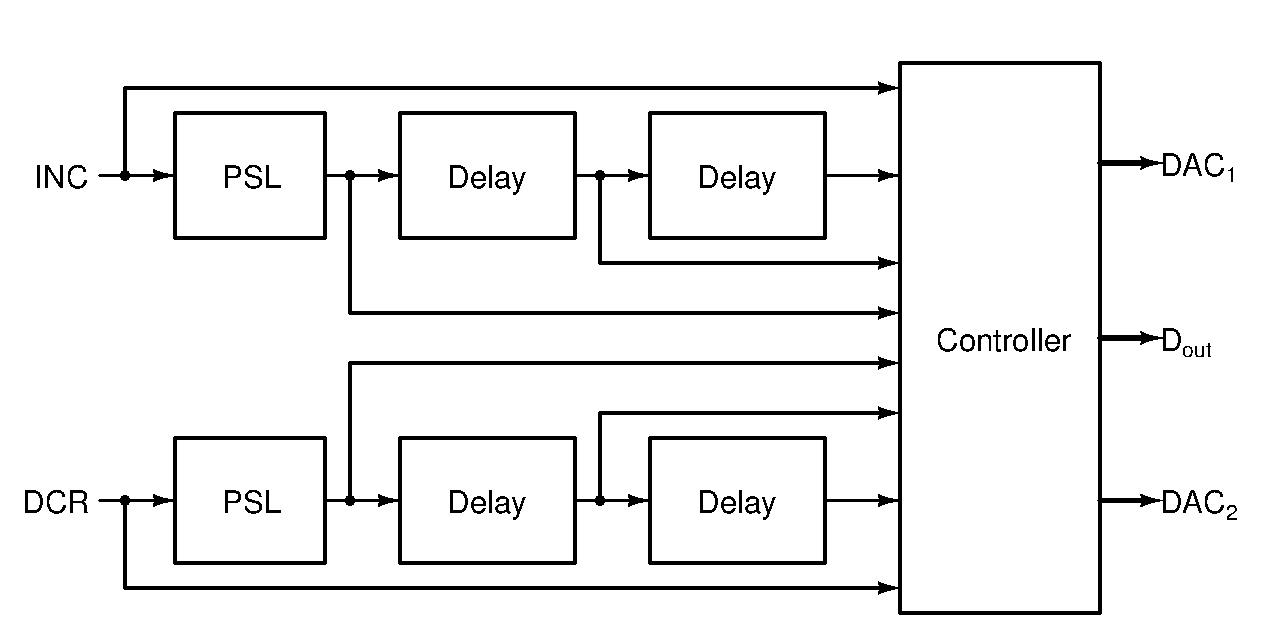
\includegraphics[scale=0.45]{./Figures/REFC.ps}
		\caption{Block Diagram of level crossing ADC.}
		\label{fig:REFC}
	\end{center}
\end{figure}

\par
\hspace{0.6cm} This technique has significant chances of misinterpreting the output when the slope of the input signal is changing. Apart from misinterpretation, the complexity of the circuit is proportional to the number of bits used to set its resolution.



 
\par
\hspace{0.6cm} The proposed architecture solves slope overloading error problem with minimal increase in complexity. The proposed technique is purely deterministic. In addition to improved performance, the proposed architecture can be reconfigured to operate in Nyquist mode. The proposed architecture also reduces power consumption when operated in Nyquist mode as compared to conventional successive approximation ADC's by reducing number of comparisions.



















